\setcounter{secnumdepth}{3} %para tener una profundidad más en las enumeraciones
\chapter{Implementaci\'on}
\label{cap:implementacion}
En el Capítulo 3 se abordó la descripción de la herramienta sin entrar en detalles de como estaba implementada, una visión general de lo que se iba a ofrecer, como la organización de los componentes, los tipos de daño o los diferentes tipos de actuadores. En este capítulo se va a tratar en profundidad la implementación de estos componentes, hablando de cómo funcionan, cómo se pueden personalizar y como los distintos componentes interactúan entre ellos.\\

La implementación de la herramienta puede encontrarse en el siguiente enlace: \href{https://github.com/CristinaMora/EnemyBehaviourFramework-2D.git}{https://github.com/CristinaMora/EnemyBehaviourFramework-2D.git}.

\section{Tecnología utilizada}
En este capítulo se describe el desarrollo de una herramienta diseñada para facilitar la creación y configuración de enemigos en un entorno 2D dentro del motor Unity. El objetivo principal es que pueda ser utilizada por diseñadores sin necesidad de escribir ni una sola línea de código, haciendo uso exclusivamente del editor y de una interfaz visual basada en prefabs y componentes reutilizables. La herramienta se presenta como un plugin modular, intuitivo y fácilmente integrable en distintos proyectos.\\

Para su desarrollo se ha utilizado el motor Unity, introducido en el Capítulo \ref{cap:estadoDeLaCuestion}, concretamente en su versión 2022.3.18f1 (LTS). No se garantiza compatibilidad con versiones anteriores, aunque se espera que funcione correctamente en versiones posteriores, salvo cambios relevantes en la API del motor.\\

Unity ha sido elegido frente a otros motores de videojuegos por su accesibilidad, su curva de aprendizaje relativamente baja y su amplia comunidad. Estas características lo convierten en una opción ideal para que cualquier usuario, sin profundos conocimientos técnicos, pueda sacar provecho de sus funcionalidades.\\

A lo largo del desarrollo se emplean diversos recursos del propio motor, como el sistema de físicas 2D o herramientas de depuración como Gizmos. Además, la arquitectura basada en componentes de Unity favorece la modularidad del sistema, permitiendo dividir el comportamiento de los enemigos en partes independientes y reutilizables.\\

A continuación se presentará la arquitectura escogida y los principales módulos de implementación.

\section{Arquitectura del sistema}
La arquitectura de la herramienta está organizada en módulos funcionales que encapsulan distintas responsabilidades dentro del sistema. Esta organización facilita la extensibilidad, el mantenimiento y la reutilización de los distintos elementos.\\

Los principales módulos de implementación incluidos en esta arquitectura son:
\begin{itemize}
\item \textbf{Módulo de actuadores:} Ejecutan acciones concretas, como moverse, disparar o generar nuevos enemigos. 
\item \textbf{Módulo de sensores:} Detectan eventos, como la presencia del jugador o colisiones.
\item \textbf{Módulo de daño:} Permite que los enemigos reciban y hagan daño.
\item \textbf{Módulo de Máquina de Estados:} Define el comportamiento que un enemigo adopta en un momento determinado.
\item \textbf{Módulo de animaciones:} Coordina las animaciones asociadas a el estado actual del enemigo.
\item \textbf{Módulo del jugador:} Módulo que sirve para contextualizar y ver las respuesta de los enemigos a las acciones del jugador.
\end{itemize}

Además, se incluyen una serie de \textit{prefabs} preconfigurados, diseñados para acelerar la creación de enemigos con comportamientos comunes. En Unity, un \textit{prefab} es una plantilla reutilizable que agrupa un conjunto de componentes, configuraciones y objetos en una única entidad. Esto permite instanciar múltiples copias consistentes de un mismo objeto manteniendo su configuración original. Gracias a esta funcionalidad, los \textit{prefabs} permiten a los diseñadores iterar rápidamente sin necesidad de modificar el código, fomentando así la reutilización y facilitando el prototipado.\\

En resumen, se ha creado una herramienta extensible, basada en módulos bien definidos y en la arquitectura por componentes de Unity. Permite crear comportamientos complejos de forma visual, lo que facilita su uso por diseñadores sin conocimientos técnicos avanzados.\\

En las siguientes secciones se describirá en detalle cada uno de los módulos que componen esta arquitectura.

\section{Módulo de actuadores}

El módulo de actuadores es el encargado de englobar todo el comportamiento de los actuadores en la herramienta. Para una explicación detallada del diseño de este módulo, puede consultarse la Sección~\ref{subsec:acciones}, donde se aborda el sistema de actuadores en su conjunto.
\begin{figure}[t]
	\centering
	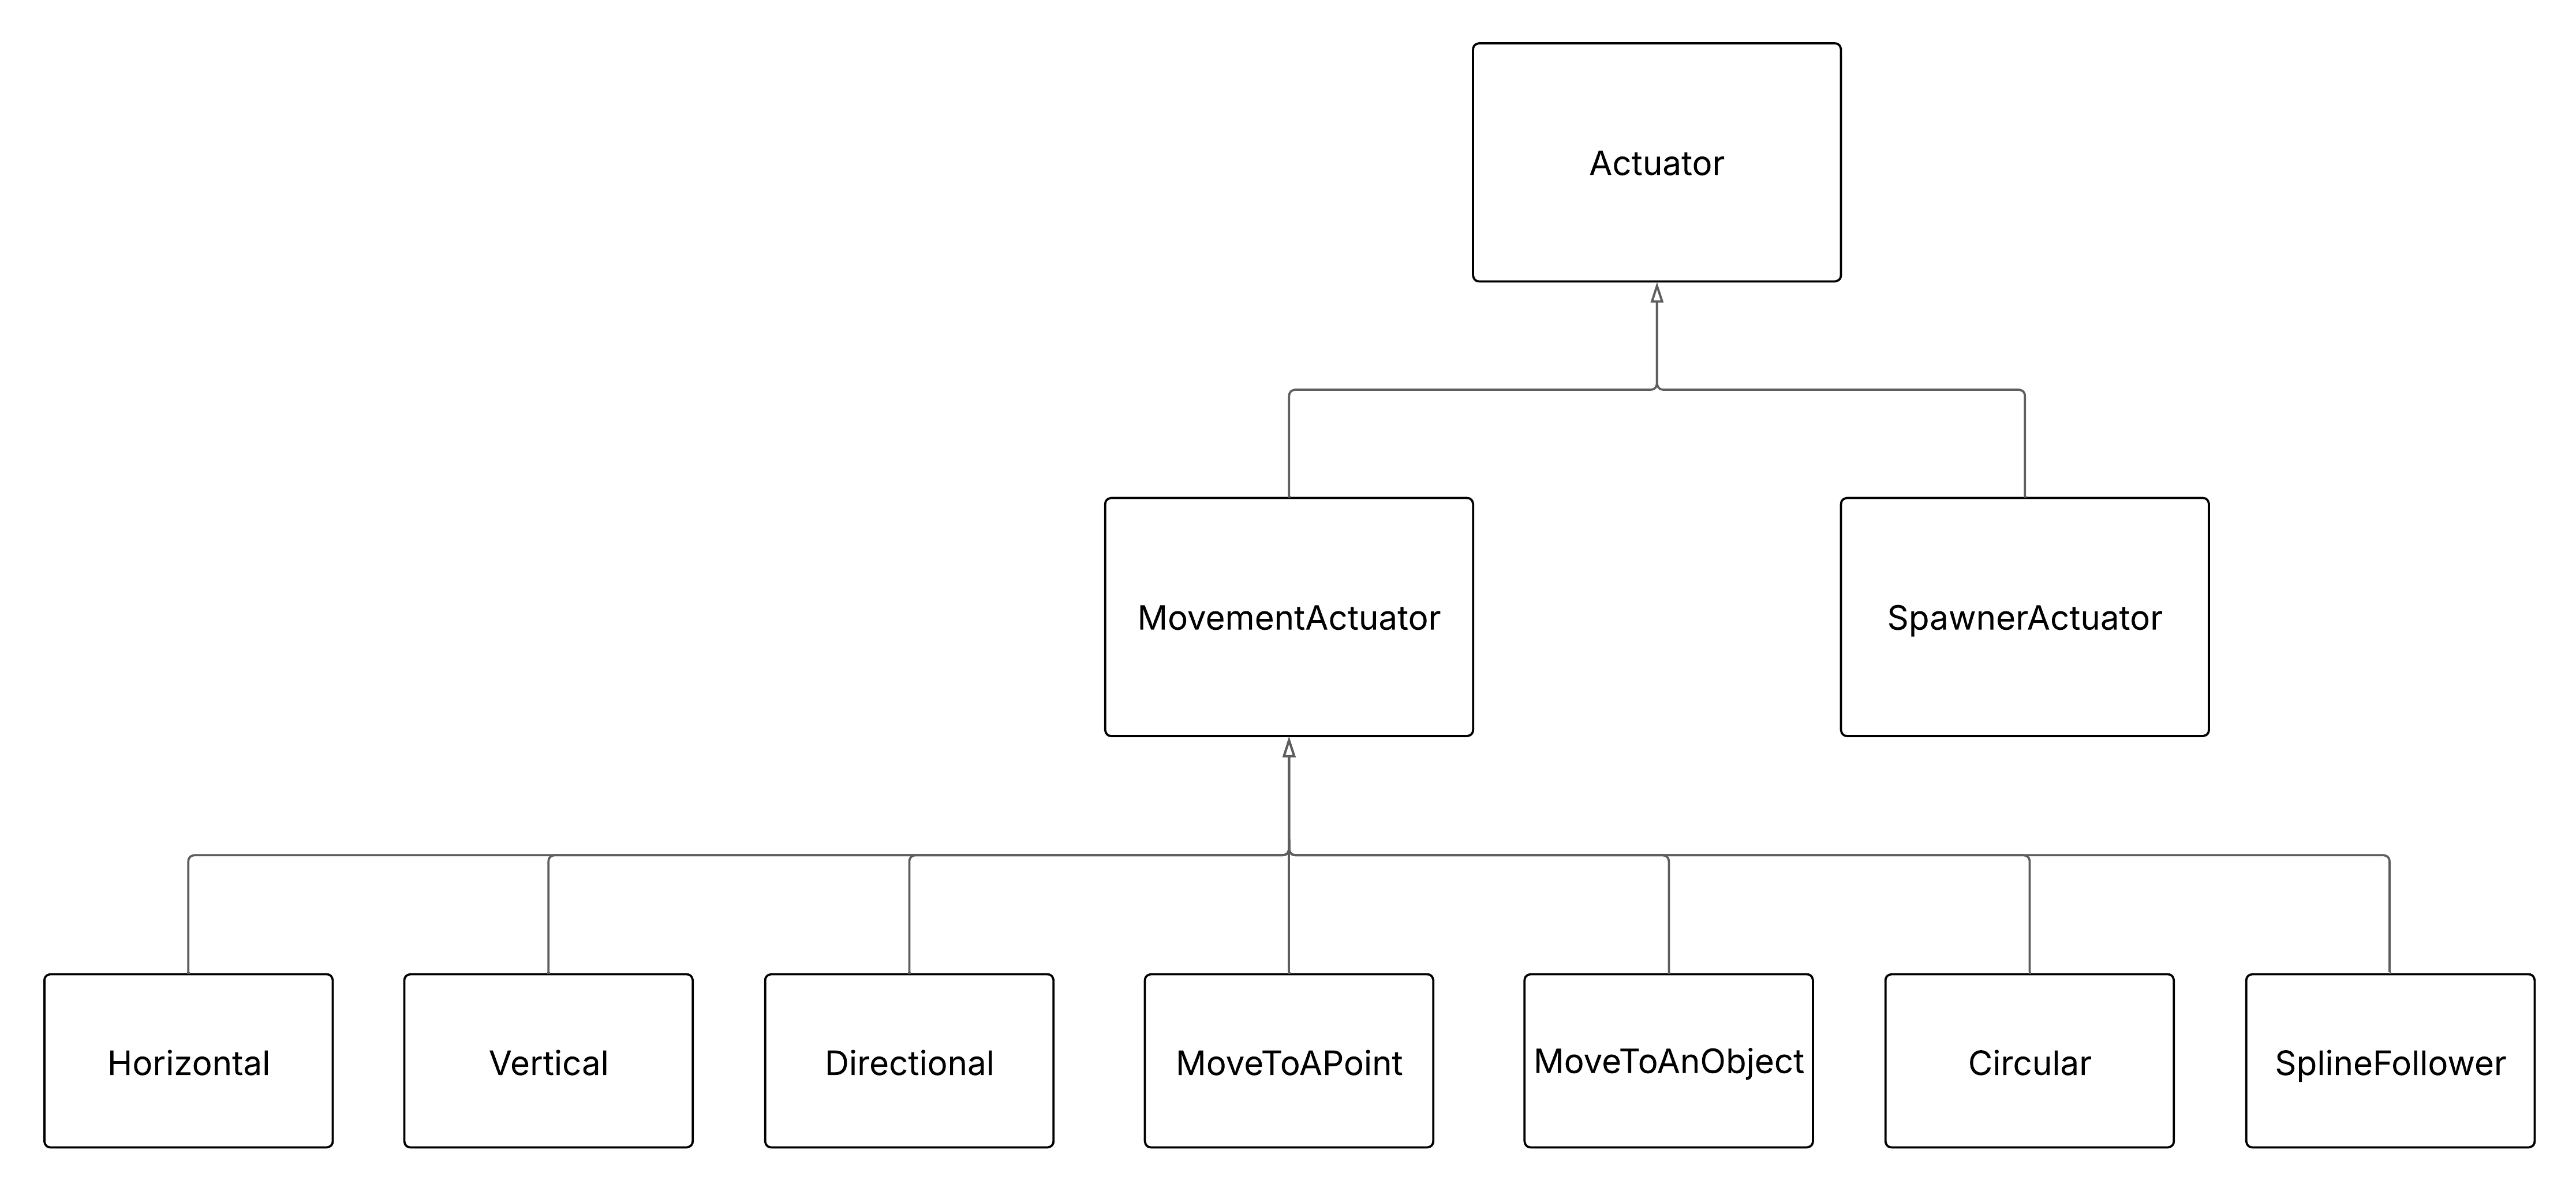
\includegraphics[width = 1\textwidth]{Imagenes/UMLActuator2.png}
	\caption{Animator Controller con sus estados y transiciones.}
	\label{fig:AnimatorController_Image}
\end{figure}


\subsection{Actuator}

La clase abstracta \texttt{Actuator} define la interfaz común para todos los actuadores del módulo. Hereda de \texttt{MonoBehaviour}, permitiendo así su uso como componente en objetos de Unity. Su principal propósito es establecer una estructura homogénea que garantice que todos los actuadores puedan ser gestionados, activados, actualizados y destruidos de forma coherente y centralizada.\\


\texttt{Actuator} declara tres métodos abstractos que deben ser implementados por todas las clases derivadas:

\begin{itemize}
\item \textbf{StartActuator()}: Método encargado de inicializar el actuador. Se invoca al comienzo de su ciclo de vida.
\item \textbf{UpdateActuator()}: Llamado una vez por frame, permite actualizar el comportamiento del actuador mientras esté activo.
\item \textbf{DestroyActuator()}: Método encargado de finalizar y limpiar los recursos asociados al actuador cuando ya no es necesario.
\end{itemize}

Además, la clase contiene una variable protegida que se puede activar o desactivar mediante el método público \textbf{SetDebug(bool debug)}.
Gracias a este diseño, se consigue una arquitectura flexible, extensible y desacoplada que facilita la incorporación de nuevos actuadores en el sistema con un esfuerzo mínimo, manteniendo siempre una interfaz común y predecible.

\subsection{MovementActuator}
La clase \texttt{Movement Actuator} que hereda de \texttt{Actuator} se usa para todos aquellos actuadores que realizan una acción de movimiento.

\textbf{Parámetros de configuración}
\begin{itemize}
	\item (bool) \textbf{Is Accelerated}: Indica si el movimiento que se va a realizar tiene una velocidad constante (valor a false), o que por el contrario, la velocidad va a ir variando (valor a true).
	\item (\texttt{EasingFunction.Ease}) \textbf{Easing Function}: Función que define cómo varía el movimiento en el tiempo. Este parámetro solo se requiere si el movimiento es acelerado.
\end{itemize}

\subsubsection{HorizontalActuator}
\texttt{Horizontal Actuator} es un actuador que hereda de \texttt{Movement Actuator} y permite mover un objeto horizontalmente, ya sea a la izquierda o a la derecha, con diferentes configuraciones de velocidad y comportamientos tras una colisión.\\

\textbf{Parámetros de configuración}
\begin{itemize}
	\item (enum) \textbf{On Collision Reaction}: Reacción que va a tener el objeto al colisionar. Puede ser \textit{None} (sin reacción), \textit{Bounce} (rebota cambiando la dirección), o \textit{Destroy} (se destruye al colisionar).
	\item (\texttt{LayerMask}) \textbf{Layers To Collide}: En caso de querer algún tipo de reacción, especificar que máscara de capas que indica cuáles son las que utilizamos para colisionar con el objeto.
	\item (enum) \textbf{Direction}: Dirección inicial del movimiento. Puede ser \textit{Left} o \textit{Right}.
	\item (float) \textbf{Speed}: Velocidad del movimiento.
	\item (float) \textbf{Goal Speed}: Velocidad final del movimiento si éste es acelerado.
	\item (float) \textbf{Interpolation Time}: Duración en segundos que va desde la velocidad inicial a \textit{Goal Speed}.
	\item (bool) \textbf{Throw}: Indica si el movimiento es un lanzamiento, es decir, se lanzará inicialmente con una velocidad inicial y, en caso contrario, se aplicará constantemente una fuerza.
	\item (bool) \textbf{Follow Player}: Determina si la dirección del movimiento se ajusta automáticamente para acercarse al jugador.
\end{itemize}

\subsubsection{VerticalActuator}
\texttt{Vertical Actuator} permite mover un objeto verticalmente, ya sea arriba o abajo, con diferentes configuraciones de velocidad y comportamientos tras una colisión.\\

\textbf{Parámetros de configuración}
\begin{itemize}
	\item (enum) \textbf{On Collision Reaction}: Reacción que va a tener el objeto al colisionar. Puede ser \textit{None} (sin reacción), \textit{Bounce} (rebota cambiando la dirección), o \textit{Destroy} (se destruye al colisionar).
	\item (\texttt{LayerMask}) \textbf{Layers To Collide}: Máscara de capas que indica cuáles son las que utilizamos para colisionar con el objeto.
	\item (enum) \textbf{Direction}: Dirección inicial del movimiento. Puede ser \textit{Up} o \textit{Down}.
	\item (float) \textbf{Speed}: Velocidad del movimiento.
	\item (float) \textbf{Goal Speed}: Velocidad final del movimiento si éste es acelerado.
	\item (float) \textbf{Interpolation Time}: Duración en segundos que va desde la velocidad inicial a \textit{Goal Speed}.
	\item (bool) \textbf{Throw}: Indica si el movimiento es un lanzamiento, es decir, se lanzará inicialmente con una velocidad inicial y, en caso contrario, se aplicará constantemente una fuerza.
	\item (bool) \textbf{Follow Player}: Determina si la dirección del movimiento se ajusta automáticamente para acercarse al jugador.
\end{itemize}

\subsubsection{DirectionalActuator}
La clase \texttt{Directional Actuator} se usa para describir un movimiento en función de un ángulo y una velocidad.\\

\textbf{Parámetros de configuración}
\begin{itemize}
	\item (\texttt{LayerMask}) \textbf{Layers To Collide}: Capas con las que puede colisionar el objeto y activar reacciones.
	\item (float) \textbf{Speed}: Velocidad del movimiento.
	\item (float) \textbf{Goal Speed}: Velocidad final del movimiento si este es acelerado.
	\item (float) \textbf{Interpolation Time}: Duración en segundos que va desde la velocidad inicial a \textit{Goal Speed}.
	\item (float) \textbf{Angle}: Ángulo de dirección del movimiento, en grados, siéndo 0º un movimiento hacía la derecha. Los grados se suman en sentido antihorario.
	\item (bool) \textbf{Throw}: Indica si el movimiento es un lanzamiento, es decir, si está a true, se lanzará inicialmente con una velocidad inicial y, en caso contrario, se aplicará constantemente una fuerza.
	\item (enum) \textbf{On Collision Reaction}: Reacción que va a tener el objeto al colisionar. Puede ser \textit{None} (sin reacción), \textit{Bounce} (rebota cambiando la dirección), o \textit{Destroy} (se destruye al colisionar).
	\item (bool) \textbf{Aim Player}: Determina si el objeto calculará automáticamente el ángulo inicial para moverse en dirección al jugador.
\end{itemize}

\subsubsection{CircularActuator}
La clase \texttt{Circular Actuator} se usa para describir un movimiento circular alrededor de un punto.\\

\textbf{Parámetros de configuración}
\begin{itemize}
	\item (float) \textbf{Angular Speed}: Velocidad de giro en grados por segundo.
	\item (\texttt{Transform}) \textbf{Rotation Point Position}: Punto central de la circunferencia que describe el objeto.
	\item (float) \textbf{Max Angle}: Ángulo máximo de giro. Si el ángulo es \textit{360º} entonces describirá una circunferencia completa, si no, hará un movimiento en forma de péndulo con los grados indicados.
	\item (float) \textbf{Angular Acceleration}: Aceleración angular.
	\item (float) \textbf{Goal Angular Speed}: Velocidad angular que se quiere alcanzar si el objeto es acelerado.
	\item (bool) \textbf{Can Rotate}: Determina si el objeto rota sobre sí mismo siguiendo la trayectoria.
	\item (float)\textbf{ Interpolation Time}: Tiempo en segundos que tarda desde la velocidad inicial hasta la velocidad final, \textit{Goal Speed}.
	\item (bool) \textbf{Point Player}: Determina si el objeto se orienta automáticamente hacia el jugador.
\end{itemize}

\subsubsection{SplineFollowerActuator}
La clase \texttt{SplineFollowerActuator} se usa para describir un movimiento mediante curvas Splines de Unity. El Actuador sigue la curva pudiendo girar el objeto a su vez.\\

\textbf{Parámetros de configuración}
\begin{itemize}
	\item (float) \textbf{Speed}: Velocidad del movimiento.
	\item (float) \textbf{Goal Speed}: Velocidad final del movimiento si este es acelerado.
	\item (float) \textbf{Interpolation Time}: Duración en segundos que va desde la velocidad inicial a \textit{Goal Speed}.
	\item (\texttt{SplineContainer}) \textbf{Spline Container}: Objeto que define una trayectoria basada en una spline, como la descrita en la \autoref{act:splinefollower}. Este componente permite establecer una serie de puntos de control conectados por curvas suaves, editables directamente en el editor de Unity. Además, el \texttt{SplineContainer} ofrece funciones para acceder a la curva en tiempo real, interpolar posiciones a lo largo del recorrido y orientar el objeto dinámicamente durante su desplazamiento.
	\item (enum) \textbf{Teleport To Closest Point}: Define cómo se ajusta el objeto a la spline al iniciarse el movimiento. Puede tener dos valores:
	\begin{itemize}
		\item \textbf{Move Enemy To Spline}: El enemigo se teletransporta a la spline.
		\item \textbf{Move Spline To Enemy}: La spline se desplaza para alinearse con la posición actual del objeto.
	\end{itemize}
\end{itemize}

\subsubsection{MoveToAPointActuator}
La clase \texttt{Move To A Point Actuator} se usa para mover el objeto en dirección a un punto no actualizable. Puede ser a un punto concreto y seguir una lista de ellos o a puntos aleatorios dentro de un área (descripción completa en Sección~\ref{sec:MoveToAPoint}.\\
Dado que la clase tiene dos maneras de funcionar y dos configuraciones distintas, primero se abordarán los parámetros de configuración comunes entre ambas y luego los parámetros específicos de cada configuración.\\

\textbf{Parámetros de configuración comunes}
\begin{itemize} 
	\item (enum) \textbf{Mode}: Define si se va a seguir una ruta por puntos (\textit{Waypoint}) o si se escogen puntos aleatoriamente dentro de una zona (\textit{RandomArea}).
\end{itemize}	

\textbf{Parámetros de configuración para Waypoint}
\begin{itemize} 	
	\item (bool) \textbf{Loop}: Determina si al finalizar los puntos volverá al primero y el movimiento se repetirá.
	\item (bool) \textbf{All Waypoints Have The Same Data}: Determina si todos los puntos usarán la misma configuración.
	\item (List<\texttt{WaypointData}>) \textbf{Waypoints Data}: Lista de puntos que el objeto debe seguir. En este caso el struct \texttt{WaypointData} está compuesto por:
	\begin{itemize} 	
		\item (\texttt{Transform}) \textbf{Waypoint Transform}: Posición a la que se debe de llegar.
		\item (float) \textbf{Time To Reach}: Tiempo estimado para alcanzar la posición deseada.
		\item (bool) \textbf{Is Accelerated}: Si se requiere aceleración.
		\item (\texttt{EasingFunction.Ease}) \textbf{Easing Function}: Función de aceleración que describe como varía la posición del objeto con respecto al tiempo, en caso de tratarse de un movimiento acelerado.
		\item (bool) \textbf{Should Stop}: Indica si debe detenerse al llegar.
		\item (float) \textbf{Stop Duration}: Tiempo que debe durar la parada en caso de existir.
	\end{itemize}
\end{itemize}

\textbf{Parámetros de configuración para RandomArea}
\begin{itemize} 	
	\item (\texttt{Collider2D}) \textbf{Random Area}: Zona dentro de la cual se moverá el objeto si está configurado como \textit{RandomArea}. 
	\item (float) \textbf{Time Between Random Points}: Tiempo necesario, en segundos, para ir de un punto aleatorio a otro.
\end{itemize}


\subsubsection{MoveToAnObjectActuator}
La clase \texttt{Move To An Object Actuator} se usa para mover el objeto en dirección a un punto actualizable, esto implica que si el punto se mueve, el objeto actualizará la trayectoria a la nueva posición.\\

\textbf{Parámetros de configuración}
\begin{itemize} 
	\item (\texttt{Transform}) \textbf{Object Transform}: Posición del objeto destino. No se necesita la referencia al objeto en sí, ya que lo único que se va a utilizar de éste es su posición.
	\item (float) \textbf{Time To Reach}: Tiempo necesario, en segundos, para llegar a la posición destino.
\end{itemize}

\subsection{SpawnerActuator}
La clase \texttt{SpawnerActuator} se usa para poder generar nuevos enemigos, pudiendo generar infinitos enemigos o un número definido de ellos cada cierto tiempo en un lugar predefinido.\\

\textbf{Parámetros de configuración}
\begin{itemize}
    \item (float) \textbf{Spawn Interval}: Intervalo de tiempo en segundos que tarda el objeto en volver a generar. 
    \item (bool) \textbf{Infinite Enemies}: Indica si se generarán enemigos indefinidamente. Si es verdadero, se crearán continuamente nuevos enemigos cada cierto tiempo indicado por \textit{Spawn Interval}. Si es falso, el número de spawns estará limitado por \texttt{Number of Times To Spawn}.
    \item (int) \textbf{Number Of Times To Spawn}: Número total de veces que se permitirá hacer spawn, si no es infinito.
    \item (List<\texttt{SpawnInfo}>) \textbf{Spawn Points}: Lista de elementos de tipo \texttt{Spawn Info}, clase compuesta por:
    \begin{itemize} 
	\item (\texttt{GameObject}) \textbf{Prefab To Spawn}: Objeto a instanciar.
	\item (\texttt{Transform}) \textbf{Spawn Point}: Punto de aparición del objeto.
    \end{itemize}
    Esta lista está diseñada para poder crear distintos tipos de enemigos o en varios sitios a la vez, dando así más flexibilidad.
\end{itemize}


\section{Módulo de sensores}
El sistema de sensores constituye un módulo independiente encargado de detectar condiciones específicas del entorno durante la ejecución del juego. Este módulo proporciona una interfaz común para diferentes tipos de sensores, permitiendo su integración flexible en otros componentes de la herramienta, como las transiciones de estado o los comportamientos de los enemigos.\\

Desde el punto de vista estructural, el módulo está diseñado siguiendo una arquitectura basada en el patrón observador (observer), lo que permite a otros componentes suscribirse a los eventos generados por los sensores sin necesidad de establecer dependencias directas.\\


Para más detalles del diseño del módulo visitar la Sección~\ref{subsec:sensores}.
La Figura~\ref{fig:UML_SensorModule} muestra el diagrama UML del módulo de sensores, en el que se puede observar la jerarquía de clases y las relaciones entre ellas. 
Para un análisis más detallado del diseño de este módulo, véase la Sección~\ref{subsec:sensores}.

\begin{figure}[t]
	\centering
	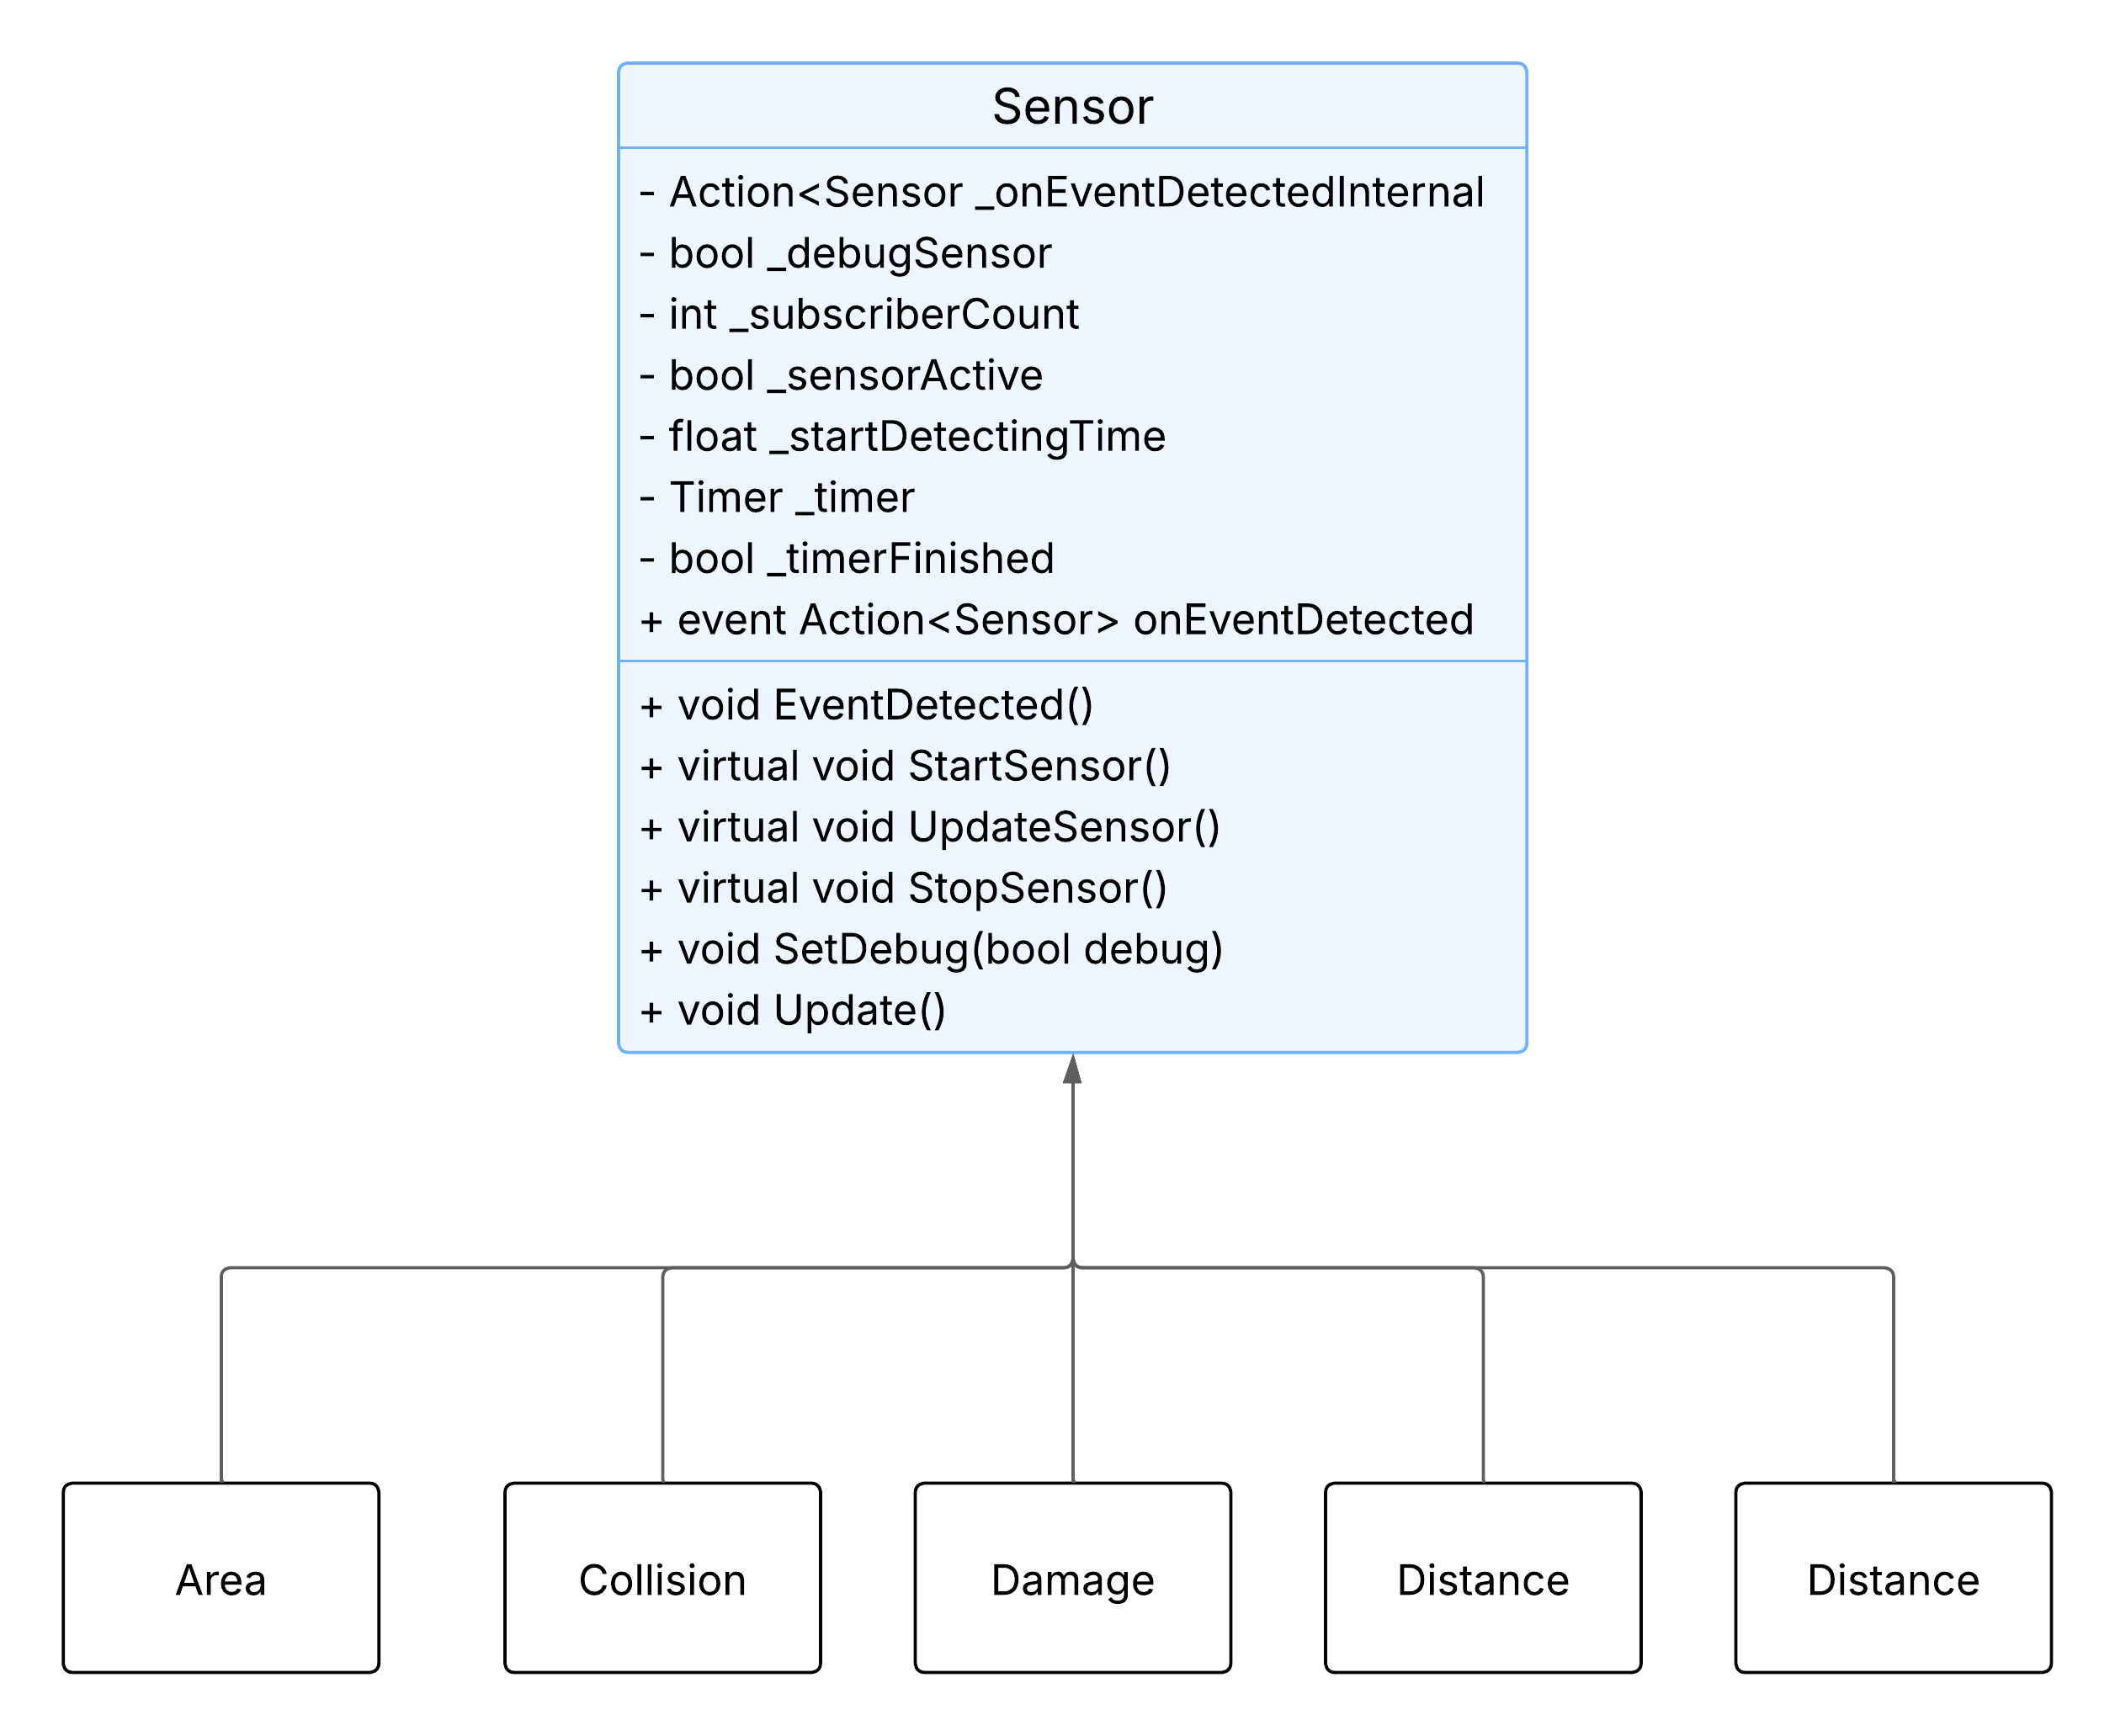
\includegraphics[width=0.75\textwidth]{Imagenes/UMLSensor.png}
	\caption{Diagrama UML del módulo de sensores.}
	\label{fig:UML_SensorModule}
\end{figure}

\subsection{Sensor}
La clase \texttt{Sensor} actúa como clase base para todos los sensores de la herramienta. Implementa una arquitectura basada en el patrón observador (observer), en la que cualquier componente interesado puede registrarse para ser notificado cuando el sensor se active.\\

Cada sensor contiene una variable de tipo \texttt{Action<Sensor>} que alberga una lista de funciones (callbacks) a ejecutar cuando se detecta una condición específica. Estas funciones pueden ser proporcionadas por otros componentes, como por ejemplo una transición que deba activarse tras la detección.\\

Para garantizar una interfaz unificada, las funciones que se registren como oyentes deben aceptar un único parámetro de tipo \texttt{Sensor}. Esto permite que, al activar el sensor, se le pueda pasar una referencia a sí mismo, facilitando que el componente suscrito acceda a su información contextual si lo necesita.\\

Este enfoque permite una arquitectura desacoplada y extensible, donde los sensores no necesitan conocer directamente qué componentes responderán a su activación, simplemente notifican a todos los suscriptores registrados.\\

Además, la implementación del sistema de eventos incluye un contador de suscriptores, que permite llevar un control sobre cuántos componentes están actualmente registrados. Esta medida ayuda a evitar errores en tiempo de ejecución relacionados con notificaciones no deseadas o fugas de memoria.\\

Cualquier clase que herede de \texttt{Sensor} tendrá la posibilidad de modificar tres funciones relativas a la lógica del sensor:

\begin{itemize}
	\item \textit{StartSensor}: Función que se encarga de activar el sensor para que se pueda comenzar a captar información y, en caso de querer un tiempo de espera al inicio de la activación, se crea el \textit{timer} correspondiente.
	\item \textit{UpdateSensor}: Función llamada en cada bucle y encargada de actualizar el tiempo que queda por esperar en caso de que el \textit{timer} no haya acabado.
	\item \textit{StopSensor}: Función que desactiva el sensor.
\end{itemize}
Estas funciones gestionan el estado interno del sensor. Una de las variables indica si el sensor se encuentra activo o inactivo, mientras que otra se utiliza para facilitar la depuración, mostrando información útil sobre su estado actual.\\

\textbf{Parámetros de configuración}
\begin{itemize}
	\item (float) \textbf{Start Detecting Time}: Tiempo que necesitará el sensor para encenderse al entrar en el estado que lo alberga. Si el sensor no está encendido se considera que está apagado y su funcionalidad quedará suspendida hasta que esté encendido.
\end{itemize}

A continuación se enumerarán y explicarán los tipos de sensores incluidos en la herramienta.\\

\subsection{AreaSensor}

\texttt{AreaSensor} representa un tipo de sensor espacial que detecta la presencia de un objeto objetivo dentro de una zona delimitada (\autoref{fig:AreaSensor_Image}). Está pensado para funcionar con zonas de activación, por lo que requiere que el objeto que lo contiene tenga un componente \texttt{Collider2D}.\\

La detección se realiza mediante los métodos \textit{OnTriggerEnter/Stay/Exit2D} provistos por \textit{Unity}. 
El primero detecta la entrada del objetivo en la zona, mientras que el segundo permite capturar situaciones en las que el objetivo ya se encuentra dentro del área al momento de encenderse el sensor. Esto evita perder eventos relevantes si la detección no estaba habilitada previamente.\\

\textbf{Parámetros de configuración}
\begin{itemize}
	\item (\texttt{GameObject}) \textbf{Target}: Objeto que se quiere detectar dentro de la zona delimitada por el Collider2D.
\end{itemize}

\begin{figure}[t]
		\centering
		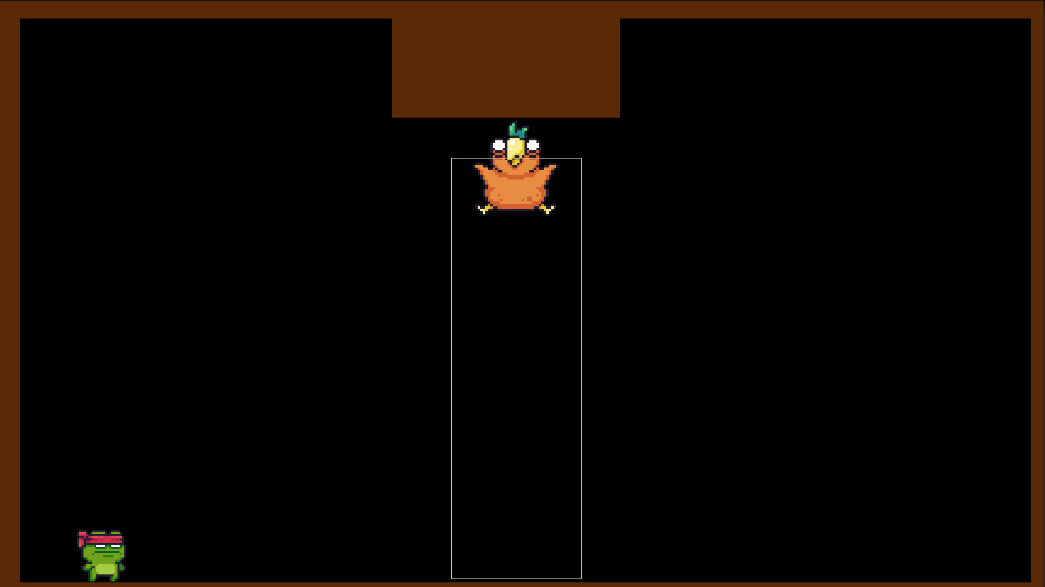
\includegraphics[width = 0.7\textwidth]{Imagenes/AreaSensor_Image.png}
		\caption{AreaSensor utilizado para enemigo que cae al detectar al jugador.}
		\label{fig:AreaSensor_Image}
\end{figure}
\subsection{CollisionSensor}
\texttt{CollisionSensor} es el sensor encargado de detectar colisiones entre el objeto que lo contiene y un conjunto específico de objetos definidos mediante una \texttt{LayerMask} de Unity. Al igual que el \texttt{AreaSensor}, este sensor requiere obligatoriamente la presencia de un componente \texttt{Collider2D} en el objeto. Para garantizarlo, se utiliza la anotación correspondiente en Unity que fuerza su inclusión automáticamente.\\

La detección de colisiones se realiza mediante los métodos \textit{OnCollisionEnter2D} y \textit{OnCollisionStay2D}. Este último es necesario para cubrir casos en los que la colisión ya se está produciendo cuando el sensor se enciende: si se utilizara únicamente \textit{OnCollisionEnter2D}, dichas situaciones no serían detectadas. Para que la colisión sea válida, es importante que ninguno de los dos objetos involucrados debe ser trigger.


\textbf{Parámetros de configuración}
\begin{itemize}
	\item (\texttt{LayerMask}) \textbf{Layers To Collide}: Máscara de capas físicas que, en caso de colisión, activarán el sensor.
\end{itemize}


\subsection{DistanceSensor}

\texttt{DistanceSensor} es el sensor utilizado para medir la distancia entre dos puntos. La distancia se medirá tomando de referencia las posiciones de sendos objetos, uno de ellos el que posee este componente y el otro el objetivo de la medición.\\

El funcionamiento del sensor dependerá del valor asignado a la variable \textit{Distance Type}, la cual es de un tipo enumerado \textit{TypeOfDistance} que especifica la manera en que se calculará la distancia. Según el valor de esta variable, se requerirán distintos parámetros o configuraciones, aunque varios valores de configuración seguirán siendo necesarios independientemente de \textit{Distance Type}.\\

\textbf{Parámetros de configuración comunes}
\begin{itemize}
	\item (enum) \textbf{Distance Type}: Tipo enumerado que determinará de qué manera se mide la distancia y qué variables se necesitarán para medirla.
	\item (enum) \textbf{Detection Condition}: Tipo enumerado que determina si el sensor se activa cuando el objetivo está dentro de esa distancia o cuando está fuera de la misma.
	\item (\texttt{GameObject})\textbf{ Target}: Entidad con la que se mide la distancia.
\end{itemize}

A continuación se especificarán los valores que puede tomar el enumerado \textit{TypeOfDistance}, sus usos y las variables específicas necesarias en cada caso.\\
\begin{itemize}
	\item \textit{Magnitude}

Configuración utilizada cuando se quiere medir la distancia como magnitud, cuya representación gráfica es un círculo, como se muestra en la \autoref{fig:DistanceSensor_Magnitude}. Dependiendo del valor de la variable \textit{Detection Condition}, el sensor se activará si el objeto objetivo está dentro o fuera del círculo.\\
\begin{figure}[t]
	\centering
	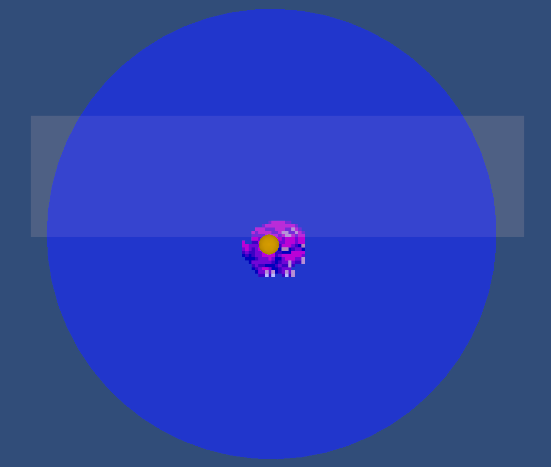
\includegraphics[width = 0.7\textwidth]{Imagenes/DistanceSensorMagnitude.png}
	\caption{Medición de distancia a través de la magnitud.}
	\label{fig:DistanceSensor_Magnitude}
\end{figure}

\textbf{Parámetros de configuración}
	\begin{itemize}
	        \item (float) \textbf{Detection Distance}: Distancia necesaria para que el sensor se active.
	 \end{itemize}

	\item \textit{Single Axis}

Con el tipo de medida \textit{Single Axis} se mide la distancia entre ambos objetos, pero solo en uno de los dos ejes: X o Y.\\
En la \autoref{fig:SingleAxis_Image} vemos un ejemplo de como luce la medición en el eje X.\\

\begin{figure}[t]
		\centering
		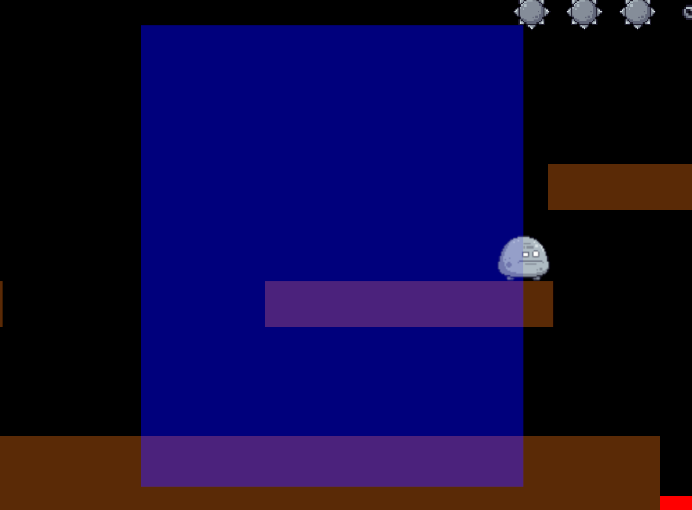
\includegraphics[width = 0.7\textwidth]{Imagenes/SingleAxis_Image.png}
		\caption{Medición de distancia en el eje X en su lado negativo.}
		\label{fig:SingleAxis_Image}
\end{figure}
\textbf{Parámetros de configuración}
	\begin{itemize}
	        \item (float) \textbf{Detection Distance}: Distancia necesaria para que el sensor se active.
	        \item (enum) \textbf{Axis}: Da opciones para escoger cuál de los dos ejes se va a medir, si X o Y.
	        \item (enum) \textbf{Detection Sides}: Permite elegir si se quiere medir la distancia a ambos lados del eje, en el lado positivo o en el lado negativo.
	 \end{itemize}
\end{itemize}

\subsection{TimeSensor}

Sensor encargado de activarse cuando pasa un tiempo determinado desde su activación. En caso de ajustar que el sensor necesitará un tiempo para encenderse, primero se procederá a medir tal tiempo y, cuando este llegue a su fin, se medirá el tiempo de activación propio del sensor.\\

\textbf{Parámetros de configuración}
	\begin{itemize}
	        \item (float) \textbf{Detection Time}: Tiempo necesario, medido en segundos, para que el sensor se active.
	 \end{itemize}

\section{Módulo de daño}
El módulo de daño es el encargado de gestionar todas las interacciones relacionadas con la aplicación y recepción de daño entre entidades del juego. Su diseño (Sección~\ref{subsec:dano}) sigue una arquitectura basada en componentes desacoplados, que permite separar claramente los elementos que emiten daño de aquellos que lo reciben.\\

Este módulo se compone principalmente de dos clases clave: \texttt{DamageEmitter} y \texttt{DamageSensor}.

\begin{figure}[t]
		\centering
		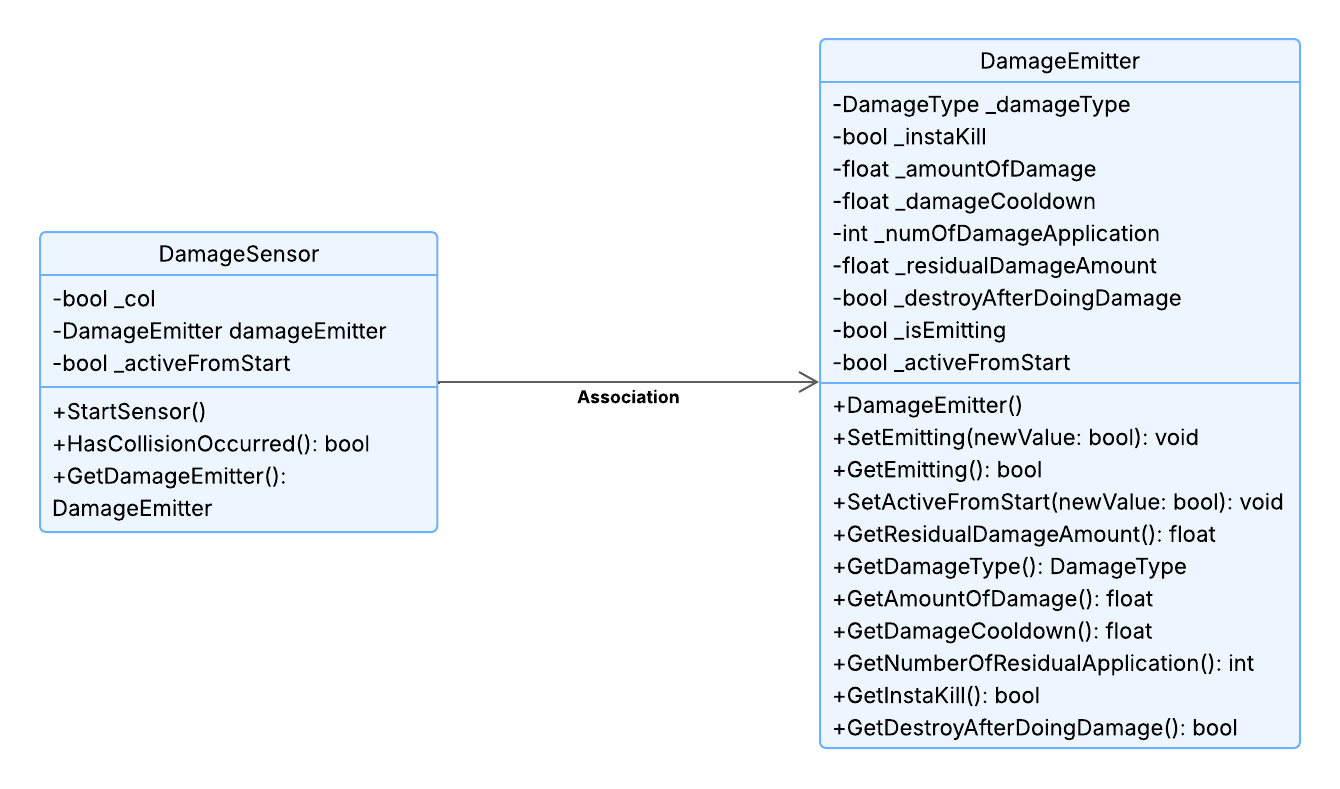
\includegraphics[width = 0.9\textwidth]{Imagenes/DamageUML.png}
		\caption{AreaSensor utilizado para enemigo que cae al detectar al jugador.}
		\label{fig:AreaSensor_Image}
\end{figure}
\subsection{DamageEmitter}
Para que una entidad pueda emitir daño, debe tener adjunto el componente \texttt{DamageEmitter}.\\
Este componente no implementa funcionalidad adicional en su propio componente, sino que actúa como una señal para el \texttt{DamageSensor}, que será explicado en el siguiente apartado. La detección de daño por parte del sensor depende de que el objeto con el que colisiona tenga este componente adjunto.\\

La manera en la que \texttt{DamageEmitter} reporta daño dependerá de un tipo enumerado llamado \texttt{DamageType}.\\
Como valores de configuración comunes para todas las configuraciones disponibles encontramos:\\

\textbf{Parámetros de configuración comunes}
\begin{itemize}
	\item (bool) \textbf{Active From Start}: En caso de que esté desactivado, no se reportará daño a no ser que el \texttt{DamageEmitter} esté incluido en un estado.
	\item (enum) \textbf{Damage Type}: Diferentes formas de producir daño a las entidades que tengan \texttt{DamageSensor}.
\end{itemize}

A continuación se concretarán los valores que puede tomar el enumerado \texttt{DamageType}, cómo funciona cada tipo de daño y qué otros valores de configuración serán necesarios.\\

\begin{itemize}
	\item \textit{Instant}
Tipo de daño que se aplica una vez producido el contacto y que no se va a volver a aplicar hasta que ese contacto no haya finalizado y se dé uno nuevo.\\

\textbf{Parámetros de configuración}
	\begin{itemize}
	        \item (bool) \textbf{Destroy After Doing Damage}: Booleano que determina si el objeto es destruido al reportar daño.
	        \item (bool) \textbf{Instant Kill}: Determina si la entidad que reporta daño elimina a su objetivo instantáneamente.
	        \item (float) \textbf{Damage Amount}: En caso de no eliminar instantáneamente al objetivo, se especificará la cantidad de daño que se hará.
	 \end{itemize}
	\item \textit{Permanence}
El daño de permanencia es aquel que produce constantemente una entidad cada cierto tiempo. Este daño se producirá mientras dure la colisión o, en caso de que sea un trigger, la superposición.\\

\textbf{Parámetros de configuración}
	\begin{itemize}
	        \item (float) \textbf{Damage Amount}: Cantidad de daño administrada cada vez.
	        \item (float) \textbf{Damage Cooldown}: Tiempo necesario para administrar daño de nuevo, medido en segundos.
	\end{itemize}

	\item \textit{Residual}
El daño residual es aquel que produce una cantidad de daño instantáneo y, tras esto, produce un número determinado de aplicaciones de otra cantidad de daño cada cierto tiempo.\\

\textbf{Parámetros de configuración}
	\begin{itemize}
	        \item (bool) \textbf{Destroy After Doing Damage}: Booleano que determina si el objeto es destruido al reportar el daño instantáneo.
	        \item (float) \textbf{Instant Damage Amount}: Cantidad de daño administrada cuando se produce el contacto.
	        \item (float) \textbf{Residual Damage Amount}: Cantidad de daño administrada por cada aplicación de daño residual.
	        \item (float) \textbf{Damage Cooldown}: Tiempo entre aplicaciones de daño residual, medido en segundos.
	        \item (int) \textbf{Number Of Applications}: Número de veces que se aplicará el daño residual.
	\end{itemize}
\end{itemize}
\subsection{DamageSensor}

\texttt{DamageSensor} es un tipo de sensor que detecta las colisiones y entradas en el área de un objeto que emite daño. Este sensor está diseñado para funcionar tanto con colisiones como con triggers. Requiere que el objeto al que se le asigne tenga un componente \texttt{Collider2D}.\\

La funcionalidad de este sensor es doble. Además de activar transiciones, se utiliza para gestionar la lógica del componente \texttt{Life} (explicado en la Sección~\ref{sec:life}). En caso de colisión, y bajo ciertas condiciones, como colisionar con un objeto que tenga el componente \texttt{DamageEmitter}, el sensor se activa. Luego, desde el componente \texttt{Life}, se gestiona qué hacer en función de las características del \texttt{DamageEmitter}.\\

Dado que \texttt{Life} es un componente utilizado para contextualizar la herramienta, pero no necesariamente el único componente de vida posible, \texttt{DamageSensor} puede utilizarse para crear nuevos componentes de vida con distintas características, separando así la funcionalidad de ambos componentes.\\

El sensor puede ser configurado para que se active desde el inicio mediante el atributo \textit{Active From Start}, lo que permite que el sensor sea útil en caso de que no se quiera que el sensor esté implicado en ninguna transición, pero sí en el sistema de gestión de salud.\\

El sensor detecta las entradas y salidas de objetos mediante los métodos \textit{OnTriggerEnter2D}, \textit{OnTriggerExit2D}, \textit{OnCollisionEnter2D} y \textit{OnCollisionExit2D}. Este control será necesario para gestionar los distintos tipos de daños que serán abordados más adelante.\\

\textbf{Parámetros de configuración}
\begin{itemize}
	\item (bool) \textbf{Active From Start}: Si es verdadero, el \textit{DamageSensor} no tendrá por qué ser incluido en ninguna transición para que este se considere activo.
\end{itemize}

\section{Módulo de Máquina de Estados}

El módulo de Máquina de Estados es el encargado de gestionar el comportamiento dinámico de una entidad. Está basado en una Máquina de Estados Finita (FSM, por sus siglas en inglés), en la que el comportamiento se estructura mediante un conjunto de \texttt{States} y transiciones (\texttt{Transitions}) entre ellos. Este módulo permite definir de forma clara y modular los distintos estados que una entidad puede tener, así como las condiciones necesarias para cambiar de uno a otro. 

Para detalles del diseño visitar la Sección~\ref{sec:fsm}.

Para una mejor organización y escalabilidad, este módulo se compone de las siguientes clases: \texttt{FSM}, \texttt{State} y \texttt{Transition}. 

\subsection{FSM}

La clase \texttt{FSM} representa la máquina de estados finita propiamente dicha. Se encarga de mantener el estado actual de la entidad, actualizarlo, y gestionar los posibles cambios de estado de manera segura. La comprobación de transiciones se realiza en el método \texttt{LateUpdate}, una vez finalizadas todas las actualizaciones del estado, para evitar cambios prematuros durante el ciclo de actualización.

\textbf{Parámetros de configuración}
\begin{itemize}
	\item (\texttt{State}) \textbf{Initial State}: Estado inicial de la máquina de estados.
\end{itemize}

\subsection{Transition}
Esta clase representa una transición de estado. Está compuesta por un sensor y un estado objetivo.Si el sensor se activa, la entidad cambiará automáticamente al estado especificado.\\

\textbf{Parámetros de configuración}
\begin{itemize}
	\item (\texttt{Sensor}) \textbf{Sensor}: Sensor encargado de detectar el evento que hará que se produzca el cambio de estado.
	\item (\texttt{State}) \textbf{Target State}: Estado de destino de la transición.
\end{itemize}

\subsection{State}

La clase \texttt{State} representa un estado de comportamiento de un enemigo. Para ello gestiona dos elementos fundamentales: \texttt{Actuators} y \texttt{Sensors}.\\
\textbf{Parámetros de configuración}
\begin{itemize}
	\item (List<\texttt{Actuator}>) \textbf{Actuator List}: Lista de Actuators que son actualizados en cada bucle y representan acciones.
	\item (List<\texttt{Transition}>) \textbf{Transition List}: Lista de Tansitions que pueden ser activadas.
	\item (List<\texttt{DamageEmitter}>) \textbf{Damage Emitter in State}: Lista de DamageEmitter activos en el estado
	\item (bool) \textbf{Debug State}: Booleano utilizado para indicar si se quiere que los Actuators en \textit{Actuator List} y Sensores en \textit{Transition List} muestren información a través del Gizmos.
\end{itemize}
Cuando se produce un cambio de estado, todos los actuadores y sensores se detienen, y los sensores se desuscriben de todas las transiciones a los que estuvieran vinculados.\\

\section{Módulo de Animación} \label{sec:animation}

El módulo de animación se encarga de coordinar la representación visual del comportamiento de los enemigos, sincronizando sus animaciones con su lógica interna. Este módulo permite adaptar dinámicamente las animaciones en función de factores como la velocidad de movimiento, la dirección, o eventos del juego como recibir daño o morir.\\

El sistema se basa en el uso del componente \texttt{Animator} de Unity, que a su vez está asociado a un \texttt{Animator Controller}. Este controlador define una Máquina de Estados Finita (FSM) visual, donde cada estado representa una animación concreta (por ejemplo: caminar, aparecer, atacar, morir) y las transiciones entre estos estados se activan mediante parámetros. Estos parámetros pueden ser booleanos, numéricos, o de tipo \textit{trigger}, y son gestionados por el módulo en tiempo de ejecución.\\

Este módulo proporciona una interfaz común para vincular las animaciones con otros módulos, como los actuadores de movimiento o el módulo de daño, de forma desacoplada y escalable.

Para más detalle del diseño de la lógica de animaciones consultar Sección~\ref{subsec:animaciones_fsm}.

\subsection{AnimatorManager}

La clase \texttt{AnimatorManager} encapsula toda la lógica necesaria para actualizar los parámetros del \texttt{Animator} de forma dinámica. Su objetivo es reflejar correctamente el comportamiento del enemigo en la animación visual que se muestra al jugador.

\textbf{Parámetros de configuración}
\begin{itemize}
	\item (bool) \textbf{Can Flip X}: Indica si el sprite puede voltearse horizontalmente.
	\item (bool) \textbf{Can Flip Y}: Indica si el sprite puede voltearse verticalmente. 
	\item (\texttt{SpriteRenderer}) \textbf{Sprite Renderer}: Componente de Unity encargado de representar visualmente un sprite en pantalla. Es el responsable de renderizar la imagen 2D asociada al objeto en la escena.

\end{itemize}

Unity utiliza un sistema de animaciones basado en un componente llamado \texttt{Animator}, que se asocia a un \texttt{Animator Controller}. Este controlador define una Máquina de Estados Finita (FSM) de animaciones, donde cada estado representa una animación concreta (como caminar, correr o morir) y las transiciones entre estados se controlan mediante parámetros. Estos parámetros pueden ser de distintos tipos, como booleanos, flotantes, enteros o \textit{triggers} (disparadores), y se actualizan dinámicamente desde el código para reflejar el comportamiento del objeto en tiempo real.\\

\subsubsection{Parámetros requeridos en el Animator}

Para centralizar la gestión de las animaciones, se ha creado un controlador personalizado (Figura~\ref{fig:AnimatorController_Image}), del tipo \texttt{Animator Controller}. Este controlador permite una integración fluida entre la lógica del comportamiento del enemigo y su representación visual, facilitando el mantenimiento y la ampliación del sistema.\\

El \texttt{Animator Controller} funciona como una máquina de estados de animación, donde cada estado representa una acción visual (como caminar, aparecer, recibir daño o morir), y las transiciones entre estos estados están condicionadas por parámetros que se actualizan dinámicamente desde el código.\\

Durante la ejecución del juego, se monitoriza constantemente la velocidad del objeto mediante su componente \texttt{Rigidbody2D}. Esta información se utiliza para actualizar tres parámetros del \texttt{Animator}: \textit{XSpeed}, \textit{YSpeed} y \textit{RotationSpeed}. Estos valores permiten adaptar en tiempo real la animación del enemigo: por ejemplo, mostrar una animación de correr hacia la derecha cuando la velocidad en el eje X es positiva. Además, si el enemigo cambia de dirección (por ejemplo, de izquierda a derecha), su sprite puede rotarse automáticamente para mantener la coherencia visual, siempre que esta opción haya sido habilitada mediante parámetros booleanos.\\

Por otro lado, el sistema de animaciones responde a eventos clave del juego mediante parámetros adicionales que se activan desde otros módulos del sistema:

\begin{itemize}
	\item El parámetro \textit{Follow} (bool) indica si el enemigo debe ajustar su animación al seguir a otro objeto, generalmente el jugador.
	\item La función \textit{ChangeState} modifica el estado de la FSM (máquina de estados finita), provocando potenciales cambios de animación.
	\item El trigger \textit{Spawn} se activa al instanciar el enemigo, permitiendo reproducir una animación de aparición o ejecutar lógica específica.
	\item Los triggers \textit{Damage} y \textit{Die} se activan al recibir daño o morir, lanzando las animaciones correspondientes. En el caso de muerte, el objeto se destruye al finalizar la animación.
\end{itemize}

En resumen, los parámetros utilizados por el \texttt{Animator Controller} se agrupan en tres tipos principales:

\begin{itemize}
	\item \textbf{Triggers}: \textit{Die}, \textit{Damage}, \textit{Spawn}, \textit{ChangeState}.
	\item \textbf{Bools}: \textit{Left}, \textit{Right}, \textit{Up}, \textit{Down}, \textit{Follow}, \textit{Rotating}.
	\item \textbf{Floats}: \textit{XSpeed}, \textit{YSpeed}, \textit{RotationSpeed}.
\end{itemize}

Gracias a esta estructura, se consigue una sincronización precisa entre el comportamiento interno del enemigo y su aspecto visual, ofreciendo una experiencia más inmersiva y coherente para el jugador.

\begin{figure}[t]
	\centering
	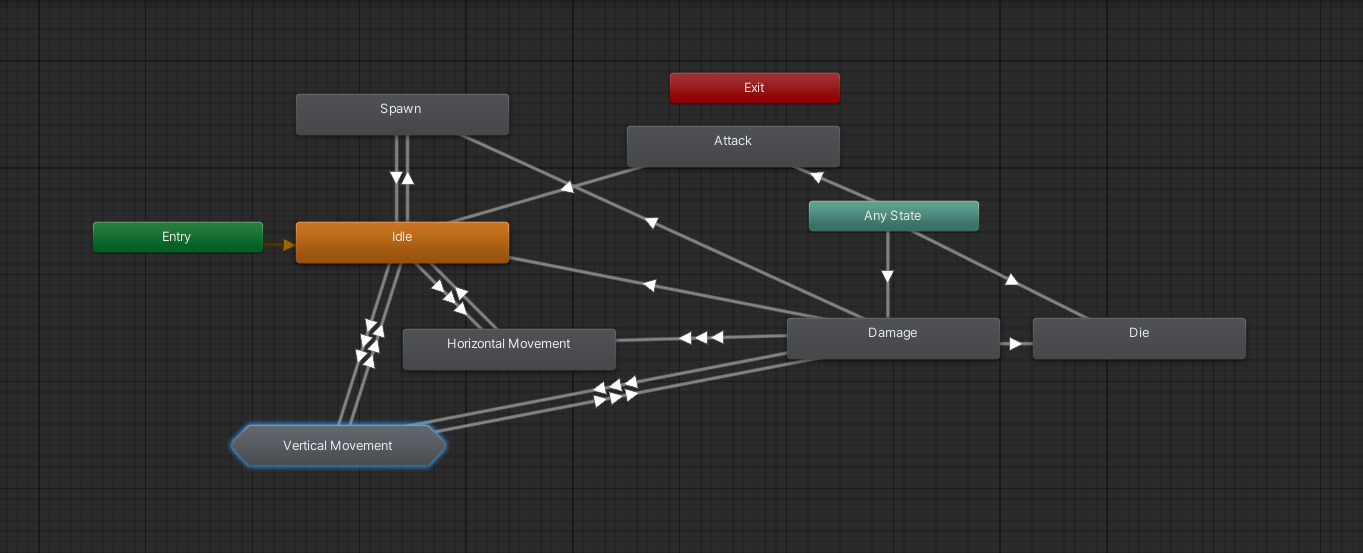
\includegraphics[width = 0.7\textwidth]{Imagenes/AnimatorController.png}
	\caption{Animator Controller con sus estados y transiciones.}
	\label{fig:AnimatorController_Image}
\end{figure}

\section{Módulo del Jugador} \label{sec:player}

El \textbf{Módulo del Jugador} encapsula toda la lógica de movimiento, interacción y control del personaje principal. Este módulo proporciona los sistemas fundamentales para el desplazamiento, salto, detección de colisiones, salud y ataques del jugador. Su implementación busca replicar una experiencia precisa y responsiva, inspirada en estándares de juegos de plataformas modernos.\\

Para lograr este comportamiento se ha tomado como referencia la implementación del canal de YouTube \textit{Mix and Jam} en su análisis del videojuego \textit{Celeste}\footnote{\url{https://www.youtube.com/watch?v=STyY26a_dPY}}, adaptando sus principios para integrarlos dentro de un sistema modular y reutilizable.

Este módulo está compuesto por varios componentes especializados que, combinados, ofrecen una experiencia de control intuitiva y sólida. En las siguientes subsecciones se detallan estos componentes, sus responsabilidades y parámetros de configuración.

\subsection{PlayerMovement}

La clase \texttt{PlayerMovement} actúa como el controlador del jugador. Su función principal es gestionar la entrada del usuario y, en consecuencia, mover al personaje. Además, si el jugador se encuentra en el suelo y se presiona la tecla de salto, la clase se encarga de ejecutar el salto.
Asimismo, maneja una situación particular en la que el jugador queda suspendido en el aire mientras se mueve hacia una pared. Si este caso no se contempla, la fuerza ejercida en el eje X puede anular la del eje Y, haciendo que el personaje quede inmóvil en una posición poco natural. Para evitar este comportamiento, si el jugador está en el aire y colisiona lateralmente con una superficie, se le fuerza a deslizarse a lo largo de esta con una velocidad constante.
Esta clase permite modificar ciertos valores como la velocidad de movimiento, la potencia de salto o la velocidad con la que el jugador se desliza por las superficies anteriormente mencionadas.\\

\textbf{Valores de configuración}
\begin{itemize}
	\item (float) \textbf{Speed}: Velocidad constante a la que se moverá el jugador.
	\item (float) \textbf{Jump Force}: Fuerza aplicada al saltar
	\item (float) \textbf{Slide Speed}: Velocidad aplicada en el eje Y cuando el jugador está en el aire y colisiona lateralmente con una superficie.
\end{itemize}

\subsection{PlayerCollisionDetection}

Este componente se encarga de detectar las colisiones del jugador. Para ello, se ajustan tres cajas de colisión (\autoref{fig:Player_Coll_Detector}): una en cada lado y otra para detectar el contacto con el suelo. Las cajas no detectan realmente colisiones, sino que comprueban si estas se superponen con alguna entidad de las capas especificadas con el método \texttt{Physics2D.OverlapBox()}.\\

\texttt{PlayerCollisionDetection} será usado por \texttt{PlayerMovement} para gestionar acciones como determinar cuándo el jugador debe deslizarse por una superficie o cuándo puede saltar.\\

\begin{figure}[t]
	\centering
	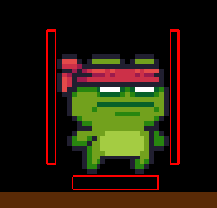
\includegraphics[width = 0.7\textwidth]{Imagenes/CollDetector.png}
	\caption{Representación de las cajas de detección de colisiones del jugador}
	\label{fig:Player_Coll_Detector}
\end{figure}

\textbf{Valores de configuración}
\begin{itemize}
	\item (bool) \textbf{ Debug Boxes}: En caso de que esta variable sea true, las cajas definidas por los campos que serán presentados a continuación serán representadas en pantalla con color rojo.
	\item (\texttt{LayerMask})  \textbf{Detection Layers}: Capas que serán tomadas en cuenta para detectar si el jugador está en el suelo o en contacto con una pared cuando está en el aire. En este caso se querrá especificar la capa que albergue a los objetos estáticos que conforman el mundo, por ejemplo \textit{World}.
	\item (\texttt{Vector2}) \textbf{Bottom/Right/Left Size}: Tamaño de las cajas.
	\item (\texttt{Vector2}) \textbf{Bottom/Right/Left Offsets}: Valores usados para reposicionar las cajas para que estén en el lugar considerado por el usuario, idealmente en los bordes del objeto.
\end{itemize}

\subsection{PlayerJump}

Para que el salto se ajuste más al estándar de los juegos de plataformas 2D, este script mejora la sensación de salto para que el personaje caiga más rápido, evitando una sensación de flotación. Además, permite realizar saltos más pequeños si el jugador suelta el botón antes.\\

Para lograrlo, el componente ajusta dos multiplicadores: uno que incrementa la gravedad cuando el jugador está cayendo y otro que reduce la altura del salto cuando este es interrumpido antes de tiempo.\\

\textbf{Parámetros de configuración}
\begin{itemize}
	\item (float) \textbf{Fall Multiplier}: Multiplicador que aumenta la gravedad cuando el personaje está cayendo, hace que el personaje caiga más rápido, dándole más peso y realismo al salto.
	\item (float) \textbf{Low Jump Multiplier}: Multiplicador que aumenta la gravedad cuando el jugador suelta el botón de salto antes de llegar al punto más alto del salto, haciendo que se puedan hacer saltos cortos, dando más control del movimiento al jugador.
\end{itemize}

\subsection{Life} \label{sec:life}

Se ha implementado una clase \texttt{Life} que gestiona los puntos de salud del objeto al que está adjunto y que se encarga de eliminar el objeto en el caso de que su vida llegue a cero. El componente pedirá al usuario un valor inicial para los puntos de vida del objeto y un valor máximo al que puede llegar la vida, para que esta sea limitada en caso de que se quiera implementar un sistema de recuperación de vida.\\

Este componente está estrechamente ligado al \texttt{DamageSensor} que detecta si ha habido una colisión con un objeto que aplique daño. Esta relación es necesaria ya que, para que se detecte el daño que decrementa la salud del objeto, se necesita este sensor, por lo que al añadir un componente \textit{Life} se añadirá este sensor automáticamente.\\

\textit{Life} diferencia entre enemigos y el jugador; en caso de que el componente esté adjunto al jugador, se deberá marcar en la opción \textit{EntityType} y el componente requerirá que se le dé la referencia a un texto del \textit{Canvas} donde se escribirá la vida actual del jugador.\\

\textbf{Parámetros de configuración}
\begin{itemize}
	\item (enum) \textbf{Entity Type}: Enumerado usado para diferenciar entre jugador y enemigos.
	\item (float) \textbf{Initial Life}: Cantidad de vida con la que inicia la entidad.
	\item (float) \textbf{Max Life}: Cantidad de vida máxima a la que puede llegar la entidad.
	\item (string) \textbf{Text Name}: En caso de ser el jugador, se pedirá un texto que precederá a los puntos de vida del jugador.
	\item (\texttt{TextMeshProUGUI}) \textbf{Life Text}: Objeto del Canvas usado para representar los puntos de vida actuales del jugador.
\end{itemize}

\subsection{PlayerDistanceAttack}

Componente encargado de representar un posible ataque a distancia del jugador. El ataque se activará con el clic izquierdo del ratón, lo que instanciará el prefab \textit{Bullet Prefab} en la posición del jugador (será importante que el objeto instanciado no pueda colisionar con el jugador, por lo que se proporciona con la herramienta un prefab llamado \texttt{PlayerBullet} que ya cumple con esta característica), el cual deberá albergar el comportamiento de una bala. La dirección que tomará la bala será aquella en la que se encuentre el cursor del ratón en el momento del clic.\\

Para evitar que el jugador pueda disparar sin restricción, se ha introducido un tiempo de espera entre disparos.\\

\textbf{Parámetros de configuración}
\begin{itemize}
	\item (\texttt{GameObject}) \textbf{Bullet Prefab}: Objeto que se instancia en la posición del jugador al hacer clic.
	\item (float) \textbf{Shooting Cooldown}: Tiempo necesario (en segundos) antes de poder disparar nuevamente.
\end{itemize}

\section {Distribución de la herramienta}

El Framework será distribuido a través de un archivo \textit{.unitypackage} descargable desde el repositorio de la herramienta.\\

Una vez descargado, el usuario podrá acceder a todo el contenido distribuido, que se detalla a continuación:\\
\begin{itemize}
\item \textbf{Animations:} Carpeta donde se encuentran tanto los \textit{sprites} usados como los \texttt{AnimatorController} creados para los enemigos de ejemplo.
\item \textbf{Materials:} En este directorio se encuentran materiales usados en la herramienta y el \texttt{Physic Material 2D} usado en algunos enemigos para mejorar su interacción con el jugador.
\item \textbf{Prefabs:} En la carpeta de \textit{Prefabs} se encuentran todos los \textit{prefabs} utilizados en la herramienta. También se encuentra el prefab \textit{BaseEnemy} el cual es usado en el manual que será mencionado luego.
\item \textbf{Scenes:} Al abrir la carpeta el usuario verá otra llamada \textit{EnemySamples} donde se encuentran todas las escenas con enemigos de ejemplo. También encontrará \textit{BaseScene} que se trata de la plantilla de escena usada en los ejemplos. Por último encontramos la escena \textit{ExampleLevel} la cual es un nivel de prueba en el que se encuentran varios enemigos en el mismo nivel.
\item \textbf{Scripts:} Por último encontramos la carpeta \textit{Scripts} en la cual encontramos:
	\begin{itemize}
	\item \textbf{Actuators:} Directorio en el cual se pueden encontrar todos los componentes relacionados con los \texttt{Actuators}.
	\item \textbf{Animations:} Aquí se encuentra el componente \texttt{AnimatorManager}.
	\item \textbf{Editor:} En esta carpeta están todos los componentes relacionados con los editores, todos ellos heredan de la clase de \textit{Unity} llamada \texttt{Editor}.
	\item \textbf{FSM:} Carpeta en la que se encuentran los componentes \texttt{State} y \texttt{FSM}.
	\item \textbf{Player Behaviour:} Lugar donde se encuentran todos los componente que tienen que ver con el funcionamiento del jugador.
	\item \textbf{SensorsAndEmitter}: Carpeta en la que están todos los componentes que heredan de \texttt{Sensor} (incluyéndolo) y \texttt{DamageEmitter}.
	\item \textbf{Otros componentes:} También se pueden encontrar los componentes: \texttt{EasingFunctions}, \texttt{Life} y \texttt{Timer}.
	\end{itemize}
\end{itemize}

Junto con el Framework, se incluye un manual de uso: \href{https://github.com/CristinaMora/EnemyBehaviourFramework-2D/tree/c1faf3195c68eb55e0c9239c02ca077aac270f7c} que contiene imágenes adicionales y está orientado a diseñadores de videojuegos. También se proporcionan una serie de tutoriales para reproducir algunos de los enemigos incluidos en el Framework.


\section{Conclusiones del Módulo de Implementación}

En este capítulo se ha detallado la construcción práctica de la herramienta, materializando el diseño teórico en un plugin de Unity modular, escalable y orientado a usuarios no programadores. A continuación, se resumen los principales logros y aprendizajes:

\begin{itemize}
	\item \textbf{Tecnología y arquitectura:} La elección de Unity 2022.3.18f1 LTS como motor base ha permitido aprovechar plenamente su sistema de componentes, prefabs y \texttt{MonoBehaviour}, garantizando compatibilidad futura y un entorno conocido para diseñadores y desarrolladores.
	\item \textbf{Módulo de actuadores:} Se implementó la clase abstracta \texttt{Actuator} y sus subtipos (\texttt{MovementActuator}, \texttt{SpawnerActuator}, etc.), permitiendo definir acciones diversas (movimiento con easing, generación de entidades) de forma coherente y reutilizable.
	\item \textbf{Módulo de sensores:} La jerarquía de \texttt{Sensor} (área, colisión, distancia y tiempo) facilita la detección de condiciones de juego mediante un patrón observador. Cada sensor notifica a las transiciones asociadas sin acoplamiento directo, potenciando la extensibilidad.
	\item \textbf{Módulo de daño:} Se separaron los roles de \texttt{DamageEmitter} y \texttt{DamageSensor}, regulando la emisión y recepción de daño de forma independiente y permitiendo integraciones limpias con sistemas de vida o efectos especiales.
	\item \textbf{Módulo de Máquina de Estados Finita:} La introducción de la clase \texttt{FSM} junto a \texttt{State} y \texttt{Transition} ha proporcionado un orquestador central para combinar sensores y actuadores en comportamientos coherentes, con cambios de estado controlados en \texttt{LateUpdate} para evitar inconsistencias en la lógica.
	\item \textbf{Módulo de animación:} Con \texttt{AnimatorManager} se ha logrado sincronizar los parámetros de movimiento, rotación y eventos (\textit{Spawn}, \textit{Damage}, \textit{Die}, \textit{ChangeState}) con un \texttt{Animator Controller}, garantizando coherencia visual entre la lógica de IA y las animaciones.
	\item \textbf{Módulo del jugador:} Se proporcionaron componentes auxiliares para movimiento (\texttt{PlayerMovement}), detección de colisiones (\texttt{PlayerCollisionDetection}), salto mejorado (\texttt{PlayerJump}), gestión de vida (\texttt{Life}) y ataque a distancia (\texttt{PlayerDistanceAttack}), cubriendo necesidades comunes de juego 2D y demostrando la flexibilidad del framework.
	\item \textbf{Distribución:} El empaquetado como plugin de Unity y la inclusión de un manual visual y de código de ejemplo facilitan su adopción en proyectos reales sin requerir modificaciones internas, cumpliendo el objetivo de accesibilidad para diseñadores.
\end{itemize}

En conjunto, el módulo de implementación ha validado la viabilidad del diseño conceptual: se ha construido una herramienta que, mediante una estructura modular y basada en patrones de diseño claros, permite configurar comportamientos de enemigos complejos sin escribir código, integrándose de forma natural en el flujo de trabajo de Unity. La implementación ha cubierto todos los aspectos planteados (movimiento, sensores, daño, estados y animaciones) y ha sentado las bases para futuras mejoras en extensibilidad y usabilidad.
